\documentclass[ignorenonframetext,]{beamer}
\setbeamertemplate{caption}[numbered]
\setbeamertemplate{caption label separator}{: }
\setbeamercolor{caption name}{fg=normal text.fg}
\beamertemplatenavigationsymbolsempty
\usepackage{lmodern}
\usepackage{amssymb,amsmath}
\usepackage{ifxetex,ifluatex}
\usepackage{fixltx2e} % provides \textsubscript
\ifnum 0\ifxetex 1\fi\ifluatex 1\fi=0 % if pdftex
  \usepackage[T1]{fontenc}
  \usepackage[utf8]{inputenc}
\else % if luatex or xelatex
  \ifxetex
    \usepackage{mathspec}
  \else
    \usepackage{fontspec}
  \fi
  \defaultfontfeatures{Ligatures=TeX,Scale=MatchLowercase}
\fi
\usefonttheme{structurebold}
% use upquote if available, for straight quotes in verbatim environments
\IfFileExists{upquote.sty}{\usepackage{upquote}}{}
% use microtype if available
\IfFileExists{microtype.sty}{%
\usepackage{microtype}
\UseMicrotypeSet[protrusion]{basicmath} % disable protrusion for tt fonts
}{}
\newif\ifbibliography
\usepackage{color}
\usepackage{fancyvrb}
\newcommand{\VerbBar}{|}
\newcommand{\VERB}{\Verb[commandchars=\\\{\}]}
\DefineVerbatimEnvironment{Highlighting}{Verbatim}{commandchars=\\\{\}}
% Add ',fontsize=\small' for more characters per line
\usepackage{framed}
\definecolor{shadecolor}{RGB}{248,248,248}
\newenvironment{Shaded}{\begin{snugshade}}{\end{snugshade}}
\newcommand{\KeywordTok}[1]{\textcolor[rgb]{0.13,0.29,0.53}{\textbf{{#1}}}}
\newcommand{\DataTypeTok}[1]{\textcolor[rgb]{0.13,0.29,0.53}{{#1}}}
\newcommand{\DecValTok}[1]{\textcolor[rgb]{0.00,0.00,0.81}{{#1}}}
\newcommand{\BaseNTok}[1]{\textcolor[rgb]{0.00,0.00,0.81}{{#1}}}
\newcommand{\FloatTok}[1]{\textcolor[rgb]{0.00,0.00,0.81}{{#1}}}
\newcommand{\ConstantTok}[1]{\textcolor[rgb]{0.00,0.00,0.00}{{#1}}}
\newcommand{\CharTok}[1]{\textcolor[rgb]{0.31,0.60,0.02}{{#1}}}
\newcommand{\SpecialCharTok}[1]{\textcolor[rgb]{0.00,0.00,0.00}{{#1}}}
\newcommand{\StringTok}[1]{\textcolor[rgb]{0.31,0.60,0.02}{{#1}}}
\newcommand{\VerbatimStringTok}[1]{\textcolor[rgb]{0.31,0.60,0.02}{{#1}}}
\newcommand{\SpecialStringTok}[1]{\textcolor[rgb]{0.31,0.60,0.02}{{#1}}}
\newcommand{\ImportTok}[1]{{#1}}
\newcommand{\CommentTok}[1]{\textcolor[rgb]{0.56,0.35,0.01}{\textit{{#1}}}}
\newcommand{\DocumentationTok}[1]{\textcolor[rgb]{0.56,0.35,0.01}{\textbf{\textit{{#1}}}}}
\newcommand{\AnnotationTok}[1]{\textcolor[rgb]{0.56,0.35,0.01}{\textbf{\textit{{#1}}}}}
\newcommand{\CommentVarTok}[1]{\textcolor[rgb]{0.56,0.35,0.01}{\textbf{\textit{{#1}}}}}
\newcommand{\OtherTok}[1]{\textcolor[rgb]{0.56,0.35,0.01}{{#1}}}
\newcommand{\FunctionTok}[1]{\textcolor[rgb]{0.00,0.00,0.00}{{#1}}}
\newcommand{\VariableTok}[1]{\textcolor[rgb]{0.00,0.00,0.00}{{#1}}}
\newcommand{\ControlFlowTok}[1]{\textcolor[rgb]{0.13,0.29,0.53}{\textbf{{#1}}}}
\newcommand{\OperatorTok}[1]{\textcolor[rgb]{0.81,0.36,0.00}{\textbf{{#1}}}}
\newcommand{\BuiltInTok}[1]{{#1}}
\newcommand{\ExtensionTok}[1]{{#1}}
\newcommand{\PreprocessorTok}[1]{\textcolor[rgb]{0.56,0.35,0.01}{\textit{{#1}}}}
\newcommand{\AttributeTok}[1]{\textcolor[rgb]{0.77,0.63,0.00}{{#1}}}
\newcommand{\RegionMarkerTok}[1]{{#1}}
\newcommand{\InformationTok}[1]{\textcolor[rgb]{0.56,0.35,0.01}{\textbf{\textit{{#1}}}}}
\newcommand{\WarningTok}[1]{\textcolor[rgb]{0.56,0.35,0.01}{\textbf{\textit{{#1}}}}}
\newcommand{\AlertTok}[1]{\textcolor[rgb]{0.94,0.16,0.16}{{#1}}}
\newcommand{\ErrorTok}[1]{\textcolor[rgb]{0.64,0.00,0.00}{\textbf{{#1}}}}
\newcommand{\NormalTok}[1]{{#1}}
\usepackage{graphicx,grffile}
\makeatletter
\def\maxwidth{\ifdim\Gin@nat@width>\linewidth\linewidth\else\Gin@nat@width\fi}
\def\maxheight{\ifdim\Gin@nat@height>\textheight0.8\textheight\else\Gin@nat@height\fi}
\makeatother
% Scale images if necessary, so that they will not overflow the page
% margins by default, and it is still possible to overwrite the defaults
% using explicit options in \includegraphics[width, height, ...]{}
\setkeys{Gin}{width=\maxwidth,height=\maxheight,keepaspectratio}

% Prevent slide breaks in the middle of a paragraph:
\widowpenalties 1 10000
\raggedbottom

\AtBeginPart{
  \let\insertpartnumber\relax
  \let\partname\relax
  \frame{\partpage}
}
\AtBeginSection{
  \ifbibliography
  \else
    \let\insertsectionnumber\relax
    \let\sectionname\relax
    \frame{\sectionpage}
  \fi
}
\AtBeginSubsection{
  \let\insertsubsectionnumber\relax
  \let\subsectionname\relax
  \frame{\subsectionpage}
}

\setlength{\emergencystretch}{3em}  % prevent overfull lines
\providecommand{\tightlist}{%
  \setlength{\itemsep}{0pt}\setlength{\parskip}{0pt}}
\setcounter{secnumdepth}{0}
\definecolor{links}{HTML}{800080}
\hypersetup{colorlinks,linkcolor=,urlcolor=links}

\title{Web Data Collection with R}
\subtitle{Regular Expressions / RegEx - A Case Study}
\author{Peter Meißner / 2016-02-29 -- 2016-03-04 / ECPR WSMT}
\date{}

\begin{document}
\frame{\titlepage}

\begin{frame}
\tableofcontents[hideallsubsections]
\end{frame}

\section{Getting to know the page}\label{getting-to-know-the-page}

\begin{frame}[fragile]{first glance at:
\url{http://ajps.org/list-of-reviewers/}}

\begin{Shaded}
\begin{Highlighting}[]
\NormalTok{url <-}\StringTok{ "http://ajps.org/list-of-reviewers/"}
\KeywordTok{browseURL}\NormalTok{(url)}
\end{Highlighting}
\end{Shaded}

\end{frame}

\begin{frame}{getting to know the page}

\begin{itemize}
\tightlist
\item
  look at the source code (Cntr-U)
\item
  inspecting elements (Cntr-Shift-I)
\end{itemize}

\end{frame}

\begin{frame}{surprise}

\begin{itemize}
\tightlist
\item
  reviewer lists are not part of the web page but available as PDF
  downloads
\end{itemize}

\end{frame}

\section{Scraping Strategy}\label{scraping-strategy}

\begin{frame}[fragile]{getting PDFs}

\begin{enumerate}
\def\labelenumi{\arabic{enumi})}
\tightlist
\item
  download page / load into R

  \begin{itemize}
  \tightlist
  \item
    \texttt{read\_html()} \emph{{[}rvest{]}}
  \end{itemize}
\item
  extract anker nodes \texttt{\textless{}a\ ...\textgreater{}}

  \begin{itemize}
  \tightlist
  \item
    \texttt{html\_nodes(...,\ xpath=...)} \emph{{[}rvest{]}}\\
  \end{itemize}
\item
  extract \texttt{href} attribute from nodes

  \begin{itemize}
  \tightlist
  \item
    \texttt{html\_attr(...,\ "href")} \emph{{[}rvest{]}}
  \end{itemize}
\item
  filter links (keep those entailing: `review'; four digits; `pdf')

  \begin{itemize}
  \tightlist
  \item
    \texttt{str\_detect(...,\ "review.*\textbackslash{}\textbackslash{}d\{4\}.*pdf")}
    \emph{{[}stringr{]}}
  \end{itemize}
\item
  download PDFs to disk

  \begin{itemize}
  \tightlist
  \item
    \texttt{download.file(...,\ ...,\ mode="wb")} \emph{{[}utils{]}}
  \end{itemize}
\end{enumerate}

\end{frame}

\begin{frame}[fragile]{extracting information from PDF}

\begin{enumerate}
\def\labelenumi{\arabic{enumi})}
\setcounter{enumi}{5}
\tightlist
\item
  converting PDF to something we can work with

  \begin{itemize}
  \tightlist
  \item
    e.g.~Adobe Acrobat Pro

    \begin{itemize}
    \tightlist
    \item
      HTML, XML, TXT, \ldots{}\\
    \end{itemize}
  \item
    e.g.~Xpdf (\url{http://www.foolabs.com/xpdf/download.html})

    \begin{itemize}
    \tightlist
    \item
      HTML, TXT, \ldots{}
    \item
      WINDOWS: \url{http://www.foolabs.com/xpdf/download.html} - add
      install path to path variable / see:
      \url{http://www.computerhope.com/issues/ch000549.htm}
    \item
      Linux e.g.: \texttt{sudo\ apt-get\ install\ poppler-utils}
    \end{itemize}
  \end{itemize}
\item
  load into R and use Regular Expressions extract information
\end{enumerate}

\end{frame}

\section{Scraping}\label{scraping}

\begin{frame}[fragile]{getting PDFs}

\begin{Shaded}
\begin{Highlighting}[]
\CommentTok{# packages needed}
\KeywordTok{require}\NormalTok{(rvest)}
\KeywordTok{require}\NormalTok{(stringr)}
\end{Highlighting}
\end{Shaded}

\end{frame}

\begin{frame}[fragile]{getting PDFs}

\begin{Shaded}
\begin{Highlighting}[]
\CommentTok{# url with list of reviews}
\NormalTok{url <-}\StringTok{ "http://ajps.org/list-of-reviewers/"}

\CommentTok{# get page}
\NormalTok{content <-}\StringTok{ }\KeywordTok{read_html}\NormalTok{(url)}

\CommentTok{# get anker (<a href=...>) nodes via xpath}
\NormalTok{ankers  <-}\StringTok{ }\KeywordTok{html_nodes}\NormalTok{(content, }\DataTypeTok{xpath =} \StringTok{"//a"}\NormalTok{)}

\CommentTok{# get value of ankers' href attribute}
\NormalTok{hrefs   <-}\StringTok{ }\KeywordTok{html_attr}\NormalTok{(ankers, }\StringTok{"href"}\NormalTok{, }
                     \DataTypeTok{default=}\StringTok{"NO HREF IN HERE"}\NormalTok{)}
\end{Highlighting}
\end{Shaded}

\end{frame}

\begin{frame}[fragile]{getting PDFs}

\begin{Shaded}
\begin{Highlighting}[]
\CommentTok{# filter links: should entail ... }
\CommentTok{# 'review', four-digit number, 'pdf'}
\NormalTok{pdf <-}\StringTok{ }\NormalTok{hrefs[ }\KeywordTok{str_detect}\NormalTok{(hrefs, }\StringTok{"review.*}\CharTok{\textbackslash{}\textbackslash{}}\StringTok{d\{4\}.*pdf"}\NormalTok{) ]}
\NormalTok{pdf}
\end{Highlighting}
\end{Shaded}

\begin{verbatim}
## [1] "http://ajpsblogging.files.wordpress.com/2015/04/ajps-reviewers-2014.pdf"
## [2] "http://ajpsblogging.files.wordpress.com/2014/01/ajps_reviewers_2013.pdf"
## [3] "http://ajpsblogging.files.wordpress.com/2013/08/reviewers_2012.pdf"     
## [4] "http://ajpsblogging.files.wordpress.com/2013/08/reviewers_2011.pdf"     
## [5] "http://ajpsblogging.files.wordpress.com/2013/08/reviewers_2010.pdf"
\end{verbatim}

\end{frame}

\begin{frame}[fragile]{getting PDFs}

\begin{Shaded}
\begin{Highlighting}[]
\CommentTok{# names for PDFs on disk}
\KeywordTok{basename}\NormalTok{(pdf)}
\end{Highlighting}
\end{Shaded}

\begin{verbatim}
## [1] "ajps-reviewers-2014.pdf" "ajps_reviewers_2013.pdf"
## [3] "reviewers_2012.pdf"      "reviewers_2011.pdf"     
## [5] "reviewers_2010.pdf"
\end{verbatim}

\begin{Shaded}
\begin{Highlighting}[]
\KeywordTok{dirname}\NormalTok{(}\KeywordTok{dirname}\NormalTok{(}\KeywordTok{dirname}\NormalTok{(pdf)))}
\end{Highlighting}
\end{Shaded}

\begin{verbatim}
## [1] "http://ajpsblogging.files.wordpress.com"
## [2] "http://ajpsblogging.files.wordpress.com"
## [3] "http://ajpsblogging.files.wordpress.com"
## [4] "http://ajpsblogging.files.wordpress.com"
## [5] "http://ajpsblogging.files.wordpress.com"
\end{verbatim}

\begin{Shaded}
\begin{Highlighting}[]
\KeywordTok{str_extract}\NormalTok{(pdf, }\StringTok{"}\CharTok{\textbackslash{}\textbackslash{}}\StringTok{d\{4\}.pdf"}\NormalTok{)}
\end{Highlighting}
\end{Shaded}

\begin{verbatim}
## [1] "2014.pdf" "2013.pdf" "2012.pdf" "2011.pdf" "2010.pdf"
\end{verbatim}

\begin{Shaded}
\begin{Highlighting}[]
\NormalTok{pdf_names <-}\StringTok{ }\KeywordTok{str_extract}\NormalTok{(pdf, }\StringTok{"}\CharTok{\textbackslash{}\textbackslash{}}\StringTok{d\{4\}.pdf"}\NormalTok{)}
\end{Highlighting}
\end{Shaded}

\begin{Shaded}
\begin{Highlighting}[]
\CommentTok{# download pdfs}
\NormalTok{for(i in }\KeywordTok{seq_along}\NormalTok{(pdf) ) \{}
  \KeywordTok{download.file}\NormalTok{(pdf[i], pdf_names[i], }\DataTypeTok{mode=}\StringTok{"wb"}\NormalTok{)}
\NormalTok{\}}
\end{Highlighting}
\end{Shaded}

\end{frame}

\section{Transforming / Reading Data}\label{transforming-reading-data}

\begin{frame}[fragile]{transforming PDFs - function}

\begin{Shaded}
\begin{Highlighting}[]
\CommentTok{# WINDOWS: xpdf: http://www.foolabs.com/xpdf/download.html }
\CommentTok{#   add install path to path variable / see: http://www.computerhope.com/issues/ch000549.htm}
\CommentTok{# Linux: sudo apt-get install poppler-utils}
\NormalTok{pdftotext <-}\StringTok{ }\NormalTok{function(fname)\{}
  \NormalTok{fname_txt <-}\StringTok{ }\KeywordTok{str_replace}\NormalTok{(fname, }\StringTok{".pdf"}\NormalTok{, }\StringTok{".txt"}\NormalTok{)}
  \KeywordTok{system2}\NormalTok{(}\DataTypeTok{command =} \StringTok{"pdftotext"}\NormalTok{, }\DataTypeTok{args =} \NormalTok{fname)}
  \KeywordTok{return}\NormalTok{(fname_txt)}
\NormalTok{\}}
\end{Highlighting}
\end{Shaded}

\end{frame}

\begin{frame}[fragile]{transforming PDFs - execution}

\begin{Shaded}
\begin{Highlighting}[]
\CommentTok{# transform PDFs to text}
\KeywordTok{pdftotext}\NormalTok{(pdf_names[}\DecValTok{1}\NormalTok{])}
\KeywordTok{pdftotext}\NormalTok{(pdf_names[}\DecValTok{2}\NormalTok{])}
\KeywordTok{pdftotext}\NormalTok{(pdf_names[}\DecValTok{3}\NormalTok{])}
\KeywordTok{pdftotext}\NormalTok{(pdf_names[}\DecValTok{4}\NormalTok{])}
\end{Highlighting}
\end{Shaded}

\end{frame}

\begin{frame}[fragile]{loading text}

\begin{Shaded}
\begin{Highlighting}[]
\CommentTok{# laod text of PDF}
\NormalTok{text1 <-}\StringTok{ }\KeywordTok{readLines}\NormalTok{(}\StringTok{"2013.txt"}\NormalTok{, }\DataTypeTok{warn=}\OtherTok{FALSE}\NormalTok{)}
\end{Highlighting}
\end{Shaded}

\end{frame}

\begin{frame}[fragile]{first glance at text}

\begin{Shaded}
\begin{Highlighting}[]
\KeywordTok{substring}\NormalTok{(text1, }\DecValTok{1}\NormalTok{, }\DecValTok{60}\NormalTok{)[}\DecValTok{6}\NormalTok{:}\DecValTok{14}\NormalTok{]}
\end{Highlighting}
\end{Shaded}

\begin{verbatim}
## [1] "parentheses!at!the!end!of!each!reviewer’s!name!indicated!the"
## [2] "completed!in!2013.!!"                                        
## [3] "!"                                                           
## [4] "Max!!Abrahms,!Johns!Hopkins!(!2!)!"                          
## [5] "Alan!I.!Abramowitz,!Emory!University!(2!)!"                  
## [6] "James!Adams,!UC!Davis!(4)!"                                  
## [7] "Claire!L.!Adida,!UCSD!(!2!)!"                                
## [8] "Marina!Agranov!,!Caltech!(!1!)!"                             
## [9] "John!S!Ahlquist!,!University!of!Wisconsin,!Madison!(!3!)!"
\end{verbatim}

\begin{itemize}
\tightlist
\item
  some useless/wrong characters → cleansing
\item
  get rid of spaces
\item
  get rid of parantheses
\item
  information scheme is: \newline{}
  \texttt{FirstName\ Lastname,\ Institution\ (NumberOfReviews)}
\item
  followed by actual extraction
\end{itemize}

\end{frame}

\begin{frame}[fragile]{preparation}

\begin{Shaded}
\begin{Highlighting}[]
\NormalTok{text1_tmp <-}\StringTok{ }
\StringTok{  }\NormalTok{text1 %>%}\StringTok{ }
\StringTok{  }\KeywordTok{str_replace_all}\NormalTok{(}\StringTok{"[!}\CharTok{\textbackslash{}f}\StringTok{]"}\NormalTok{,}\StringTok{" "}\NormalTok{) %>%}\StringTok{   }\CommentTok{# drop form feed}
\StringTok{  }\KeywordTok{str_replace_all}\NormalTok{(}\StringTok{"}\CharTok{\textbackslash{}\textbackslash{}}\StringTok{]"}\NormalTok{,}\StringTok{" "}\NormalTok{) %>%}\StringTok{     }\CommentTok{# drop ]}
\StringTok{  }\KeywordTok{str_replace_all}\NormalTok{(}\StringTok{"}\CharTok{\textbackslash{}\textbackslash{}}\StringTok{(|}\CharTok{\textbackslash{}\textbackslash{}}\StringTok{)"}\NormalTok{, }\StringTok{""}\NormalTok{) %>%}\StringTok{ }\CommentTok{# drop ( )}
\StringTok{  }\KeywordTok{str_replace}\NormalTok{(}\StringTok{" ,"}\NormalTok{, }\StringTok{","}\NormalTok{) %>%}\StringTok{         }\CommentTok{# correct space}
\StringTok{  }\KeywordTok{str_replace_all}\NormalTok{(}\StringTok{"  "}\NormalTok{, }\StringTok{" "}\NormalTok{) %>%}\StringTok{     }\CommentTok{# correct space}
\StringTok{  }\KeywordTok{str_trim}\NormalTok{()                         }\CommentTok{# correct space}

\NormalTok{text1_tmp <-}\StringTok{ }
\StringTok{  }\NormalTok{text1_tmp[text1_tmp !=}\StringTok{ ""}\NormalTok{] }\CommentTok{# drop empty lines}

\NormalTok{text1_tmp <-}\StringTok{ }
\StringTok{  }\NormalTok{text1_tmp[-}\KeywordTok{c}\NormalTok{(}\DecValTok{1}\NormalTok{:}\DecValTok{5} \NormalTok{)]        }\CommentTok{# drop non data}
\end{Highlighting}
\end{Shaded}

\end{frame}

\begin{frame}[fragile]{cleaned up}

\begin{Shaded}
\begin{Highlighting}[]
\NormalTok{text1_tmp[}\DecValTok{1}\NormalTok{:}\DecValTok{10}\NormalTok{]}
\end{Highlighting}
\end{Shaded}

\begin{verbatim}
##  [1] "Max Abrahms, Johns Hopkins 2"                       
##  [2] "Alan I. Abramowitz, Emory University 2"             
##  [3] "James Adams, UC Davis 4"                            
##  [4] "Claire L. Adida, UCSD 2"                            
##  [5] "Marina Agranov, Caltech 1"                          
##  [6] "John S Ahlquist, University of Wisconsin, Madison 3"
##  [7] "Faisal Ahmed, Oxford University 2"                  
##  [8] "T.K. Ahn, Seoul National University 1"              
##  [9] "Ariel Ahram, Virginia Tech 1"                       
## [10] "Deniz Aksoy, Princeton University 1"
\end{verbatim}

\end{frame}

\section{First Result}\label{first-result}

\begin{frame}[fragile]{Reviewers}

\begin{Shaded}
\begin{Highlighting}[]
\KeywordTok{length}\NormalTok{(}\KeywordTok{grep}\NormalTok{(}\StringTok{"Konstanz"}\NormalTok{, text1_tmp))}
\end{Highlighting}
\end{Shaded}

\begin{verbatim}
## [1] 6
\end{verbatim}

\begin{Shaded}
\begin{Highlighting}[]
\KeywordTok{length}\NormalTok{(}\KeywordTok{grep}\NormalTok{(}\StringTok{"Harvard"}\NormalTok{, text1_tmp))}
\end{Highlighting}
\end{Shaded}

\begin{verbatim}
## [1] 24
\end{verbatim}

\begin{Shaded}
\begin{Highlighting}[]
\KeywordTok{length}\NormalTok{(}\KeywordTok{grep}\NormalTok{(}\StringTok{"Berlin"}\NormalTok{, text1_tmp))}
\end{Highlighting}
\end{Shaded}

\begin{verbatim}
## [1] 3
\end{verbatim}

\begin{Shaded}
\begin{Highlighting}[]
\KeywordTok{length}\NormalTok{(}\KeywordTok{grep}\NormalTok{(}\StringTok{"Bamberg"}\NormalTok{, text1_tmp))}
\end{Highlighting}
\end{Shaded}

\begin{verbatim}
## [1] 0
\end{verbatim}

\begin{Shaded}
\begin{Highlighting}[]
\KeywordTok{length}\NormalTok{(}\KeywordTok{grep}\NormalTok{(}\StringTok{"UCLA"}\NormalTok{, text1_tmp))}
\end{Highlighting}
\end{Shaded}

\begin{verbatim}
## [1] 2
\end{verbatim}

\end{frame}

\section{Extraction}\label{extraction}

\begin{frame}[fragile]{names}

\begin{Shaded}
\begin{Highlighting}[]
\NormalTok{names <-}\StringTok{ }
\StringTok{  }\NormalTok{text1_tmp %>%}\StringTok{ }
\StringTok{  }\KeywordTok{str_extract}\NormalTok{(}\StringTok{"^.*?,"}\NormalTok{) %>%}\StringTok{ }
\StringTok{  }\KeywordTok{str_replace_all}\NormalTok{(}\StringTok{"  |,"}\NormalTok{, }\StringTok{" "}\NormalTok{) %>%}\StringTok{ }
\StringTok{  }\KeywordTok{str_trim}\NormalTok{( )}
\KeywordTok{sample}\NormalTok{(names, }\DecValTok{10}\NormalTok{)}
\end{Highlighting}
\end{Shaded}

\begin{verbatim}
##  [1] "David Karol"           "Charles Daniel Myers" 
##  [3] "Anna Harvey"           "Kåre Vernby"          
##  [5] "Sean Cain"             "Kent Tedin"           
##  [7] "Matthew Lee Blackwell" "Amanda Driscoll"      
##  [9] "Jay Gatrell"           "Andrew Therriault"
\end{verbatim}

\end{frame}

\begin{frame}[fragile]{institutions}

\begin{Shaded}
\begin{Highlighting}[]
\NormalTok{institution <-}
\StringTok{  }\NormalTok{text1_tmp %>%}\StringTok{ }
\StringTok{  }\KeywordTok{str_extract}\NormalTok{(}\StringTok{",.*}\CharTok{\textbackslash{}\textbackslash{}}\StringTok{d"}\NormalTok{) %>%}\StringTok{ }
\StringTok{  }\KeywordTok{str_replace_all}\NormalTok{(}\StringTok{"^ ,|^,|}\CharTok{\textbackslash{}\textbackslash{}}\StringTok{d$"}\NormalTok{,}\StringTok{""}\NormalTok{) %>%}\StringTok{ }
\StringTok{  }\KeywordTok{str_trim}\NormalTok{()}
\KeywordTok{sample}\NormalTok{(institution, }\DecValTok{7}\NormalTok{)}
\end{Highlighting}
\end{Shaded}

\begin{verbatim}
## [1] "University of Wisconsin"        "Hebrew University of Jerusalem"
## [3] "Bucknell University"            "Erasmus University Rotterdam"  
## [5] "University of Mississippi"      "The World Bank"                
## [7] "University of Houston"
\end{verbatim}

\end{frame}

\begin{frame}[fragile]{reviews}

\begin{Shaded}
\begin{Highlighting}[]
\NormalTok{reviews <-}\StringTok{      }
\StringTok{  }\NormalTok{text1_tmp %>%}\StringTok{ }
\StringTok{  }\KeywordTok{str_extract}\NormalTok{(}\StringTok{"}\CharTok{\textbackslash{}\textbackslash{}}\StringTok{d+"}\NormalTok{) %>%}\StringTok{ }
\StringTok{  }\NormalTok{as.numeric }
\KeywordTok{table}\NormalTok{(reviews)}
\end{Highlighting}
\end{Shaded}

\begin{verbatim}
## reviews
##   1   2   3   4   5 
## 947 181  34   7   1
\end{verbatim}

\end{frame}

\begin{frame}[fragile]{reviews}

\begin{Shaded}
\begin{Highlighting}[]
\KeywordTok{data.frame}\NormalTok{(}\DataTypeTok{n=}\NormalTok{reviews, names, institution)[reviews >}\StringTok{ }\DecValTok{3}\NormalTok{, ]}
\end{Highlighting}
\end{Shaded}

\begin{verbatim}
##      n                 names              institution
## 3    4           James Adams                 UC Davis
## 27   4        Scott Ashworth    University of Chicago
## 541  4          Cindy D. Kam    Vanderbilt University
## 592  5         Gregory Koger      University of Miami
## 684  4         Neil Malhotra      Stanford University
## 950  4 Leslie Schwindt Bayer          Rice University
## 1095 4           Erik Voeten    Georgetown University
## 1152 4         Jonathan Woon University of Pittsburgh
\end{verbatim}

\end{frame}

\begin{frame}[fragile]{save data gathered so far}

\begin{Shaded}
\begin{Highlighting}[]
\NormalTok{revdat <-}\StringTok{ }\KeywordTok{data.frame}\NormalTok{(}
  \NormalTok{reviews, }
  \NormalTok{names, }
  \NormalTok{institution, }
  \DataTypeTok{stringsAsFactors =} \OtherTok{FALSE}
\NormalTok{)}
\KeywordTok{save}\NormalTok{(revdat, }\DataTypeTok{file =} \StringTok{"revdat.Rdata"}\NormalTok{)}
\end{Highlighting}
\end{Shaded}

\end{frame}

\section{Extension (1)}\label{extension-1}

\begin{frame}[fragile]{geocoding institutions}

\begin{Shaded}
\begin{Highlighting}[]
\KeywordTok{require}\NormalTok{(ggmap)}
\CommentTok{# geocoding takes a while -> save results}
\CommentTok{# 2500 requests allowed per day}
\NormalTok{if ( !}\KeywordTok{file.exists}\NormalTok{(}\StringTok{"scenario1_inst_geocoded_pos.rdata"}\NormalTok{))\{}
  \NormalTok{pos <-}\StringTok{ }\KeywordTok{geocode}\NormalTok{(institution)}
  \KeywordTok{geocodeQueryCheck}\NormalTok{() }
  \KeywordTok{save}\NormalTok{(pos, }\DataTypeTok{file=}\StringTok{"scenario1_inst_geocoded_pos.rdata"}\NormalTok{)}
\NormalTok{\} else \{}
  \KeywordTok{load}\NormalTok{(}\StringTok{"scenario1_inst_geocoded_pos.rdata"}\NormalTok{)}
\NormalTok{\}}
\end{Highlighting}
\end{Shaded}

\end{frame}

\begin{frame}[fragile]{plot coordinates}

\begin{Shaded}
\begin{Highlighting}[]
\NormalTok{mapWorld <-}\StringTok{ }\KeywordTok{borders}\NormalTok{(}\StringTok{"world"}\NormalTok{)}
\end{Highlighting}
\end{Shaded}

\begin{verbatim}
## 
##  # maps v3.1: updated 'world': all lakes moved to separate new #
##  # 'lakes' database. Type '?world' or 'news(package="maps")'.  #
\end{verbatim}

\begin{Shaded}
\begin{Highlighting}[]
\NormalTok{map <-}\StringTok{   }
\StringTok{  }\KeywordTok{ggplot}\NormalTok{() +}\StringTok{ }
\StringTok{  }\NormalTok{mapWorld +}\StringTok{ }
\StringTok{  }\KeywordTok{geom_point}\NormalTok{(}\KeywordTok{aes}\NormalTok{(}\DataTypeTok{x=}\NormalTok{pos$lon, }\DataTypeTok{y=}\NormalTok{pos$lat) ,}
             \DataTypeTok{color=}\StringTok{"#F54B1A90"}\NormalTok{, }\DataTypeTok{size=}\DecValTok{3} \NormalTok{,}
             \DataTypeTok{na.rm=}\NormalTok{T) +}\StringTok{ }
\StringTok{  }\KeywordTok{theme_bw}\NormalTok{() +}\StringTok{ }
\StringTok{  }\KeywordTok{coord_map}\NormalTok{(}\DataTypeTok{xlim=}\KeywordTok{c}\NormalTok{(-}\DecValTok{180}\NormalTok{, }\DecValTok{180}\NormalTok{), }\DataTypeTok{ylim=}\KeywordTok{c}\NormalTok{(-}\DecValTok{60}\NormalTok{,}\DecValTok{70}\NormalTok{))}
\end{Highlighting}
\end{Shaded}

\end{frame}

\begin{frame}[fragile]{plot coordinates}

\begin{Shaded}
\begin{Highlighting}[]
\NormalTok{map }\CommentTok{# ajps 2013 reviewers worldwide}
\end{Highlighting}
\end{Shaded}

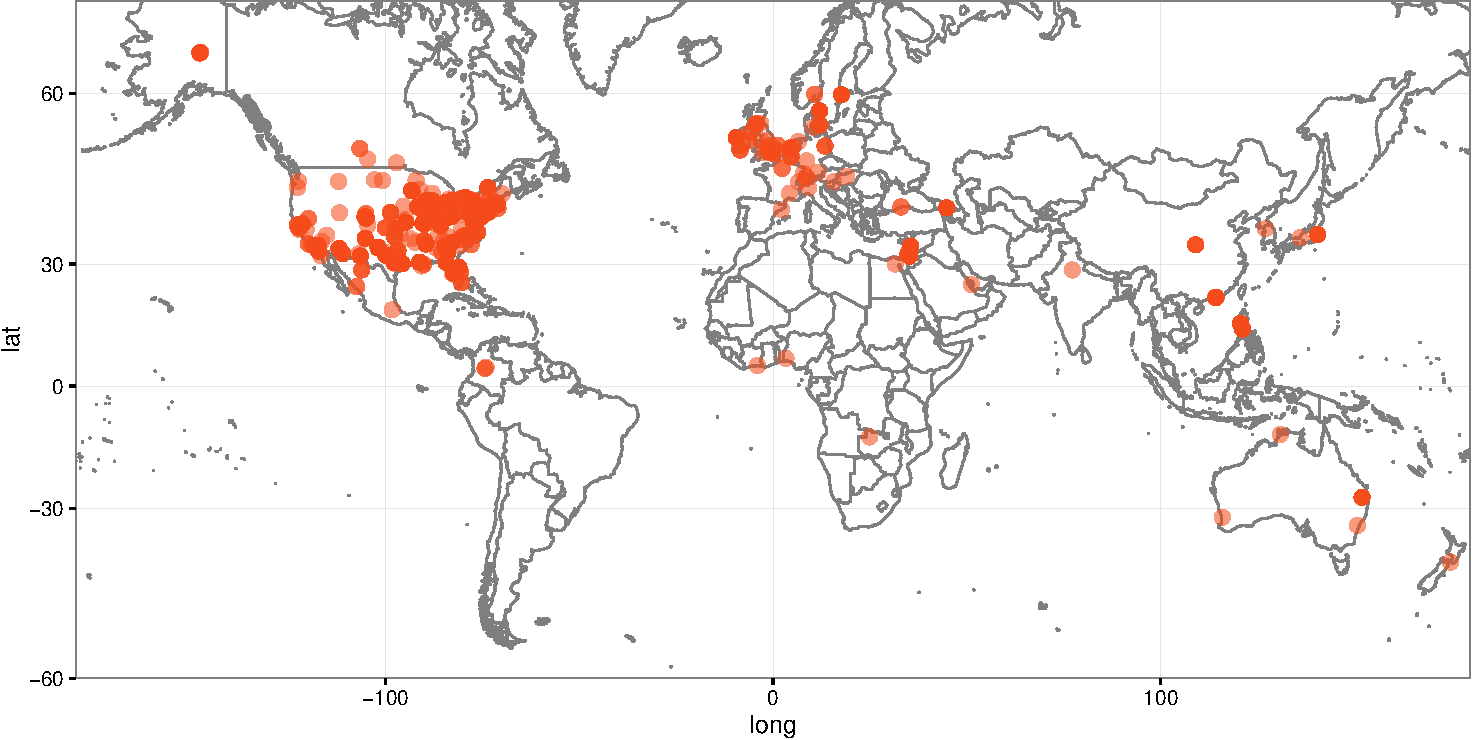
\includegraphics{regex_case_files/figure-beamer/unnamed-chunk-21-1.pdf}

\end{frame}

\begin{frame}{Extension (2)}

\begin{itemize}
\tightlist
\item
  grab articel authors for some years
\item
  and compare to reviewers
\end{itemize}

\end{frame}

\end{document}
